\subsubsection{Kartierung}
Alle Kartierungsvorgänge wurden mit der Free Open Source Software \emph{QGIS}\cite{qgis}\\durchgeführt.
\begin{figure}[ht]
    \centering
    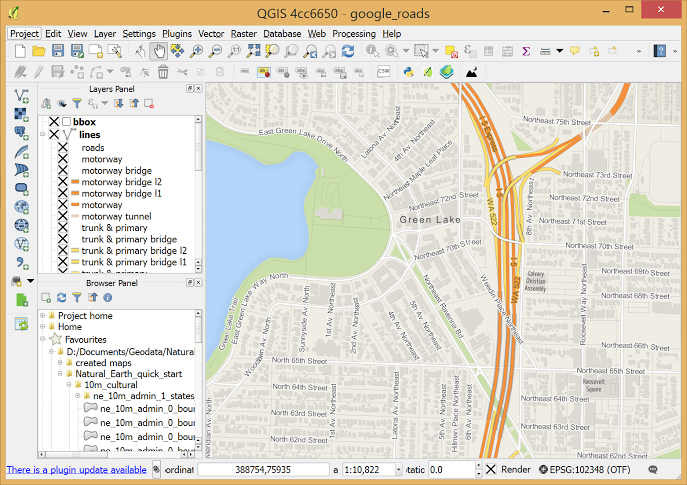
\includegraphics[width=.5\linewidth]{Bilder/QGIS/about-screenshot.png}
    \caption[fig:qgisabout]{QGIS-Benutzeroberfläche}
\end{figure}
\\Mithilfe dieser Software lassen sich basierend auf bereits existierenden Karten, 
wie beispielsweise \emph{OpenStreetMap}\cite{ostrm} oder \emph{OpenSeaMap}\cite{oseam}, eigene Routen und Points of \\Interest(POIs) ohne großen 
Aufwand eintragen. Genauso leicht erfolgt der Import sowie vom Multibeam,  als auch von den Navigationsgeräten der ALDEBARAN gespeicherten 
Positions-  und Geschwindigkeitsdaten.
\begin{figure}[ht]
    \begin{minipage}{0.48\textwidth}
        \centering
        
\includegraphics[width=.9\linewidth]{Bilder/platzhalter.jpeg}
        \caption[fig:planned_route]{Geplante Route}
    \end{minipage}
    \begin{minipage}{0.48\textwidth}
        \centering
        
\includegraphics[width=.9\linewidth]{Bilder/platzhalter.jpeg}
        \caption[fig:actual_route]{Gefahrene Route}
    \end{minipage}
\end{figure}